\chapter{Metodologia}
% Nesta seção, serão definidas as métricas específicas que serão utilizadas para avaliar a eficácia dos processamentos de imagem no estudo.

A metodologia delineada neste estudo tem como propósito fundamental o desenvolvimento de um arcabouço sistemático para aprimorar, comparar, selecionar e combinar técnicas de processamento de imagem, visando aprimorar a detecção e classificação de falhas em cadeias de isoladores. O processo é estruturado e iterativo, conforme ilustrado no fluxograma da Figura \ref{fig:fluxograma_metodologia}.

\begin{figure}[H]
    \centering
    \caption{\label{fig:fluxograma_metodologia}Fluxograma da metodologia de processamento de imagens}
    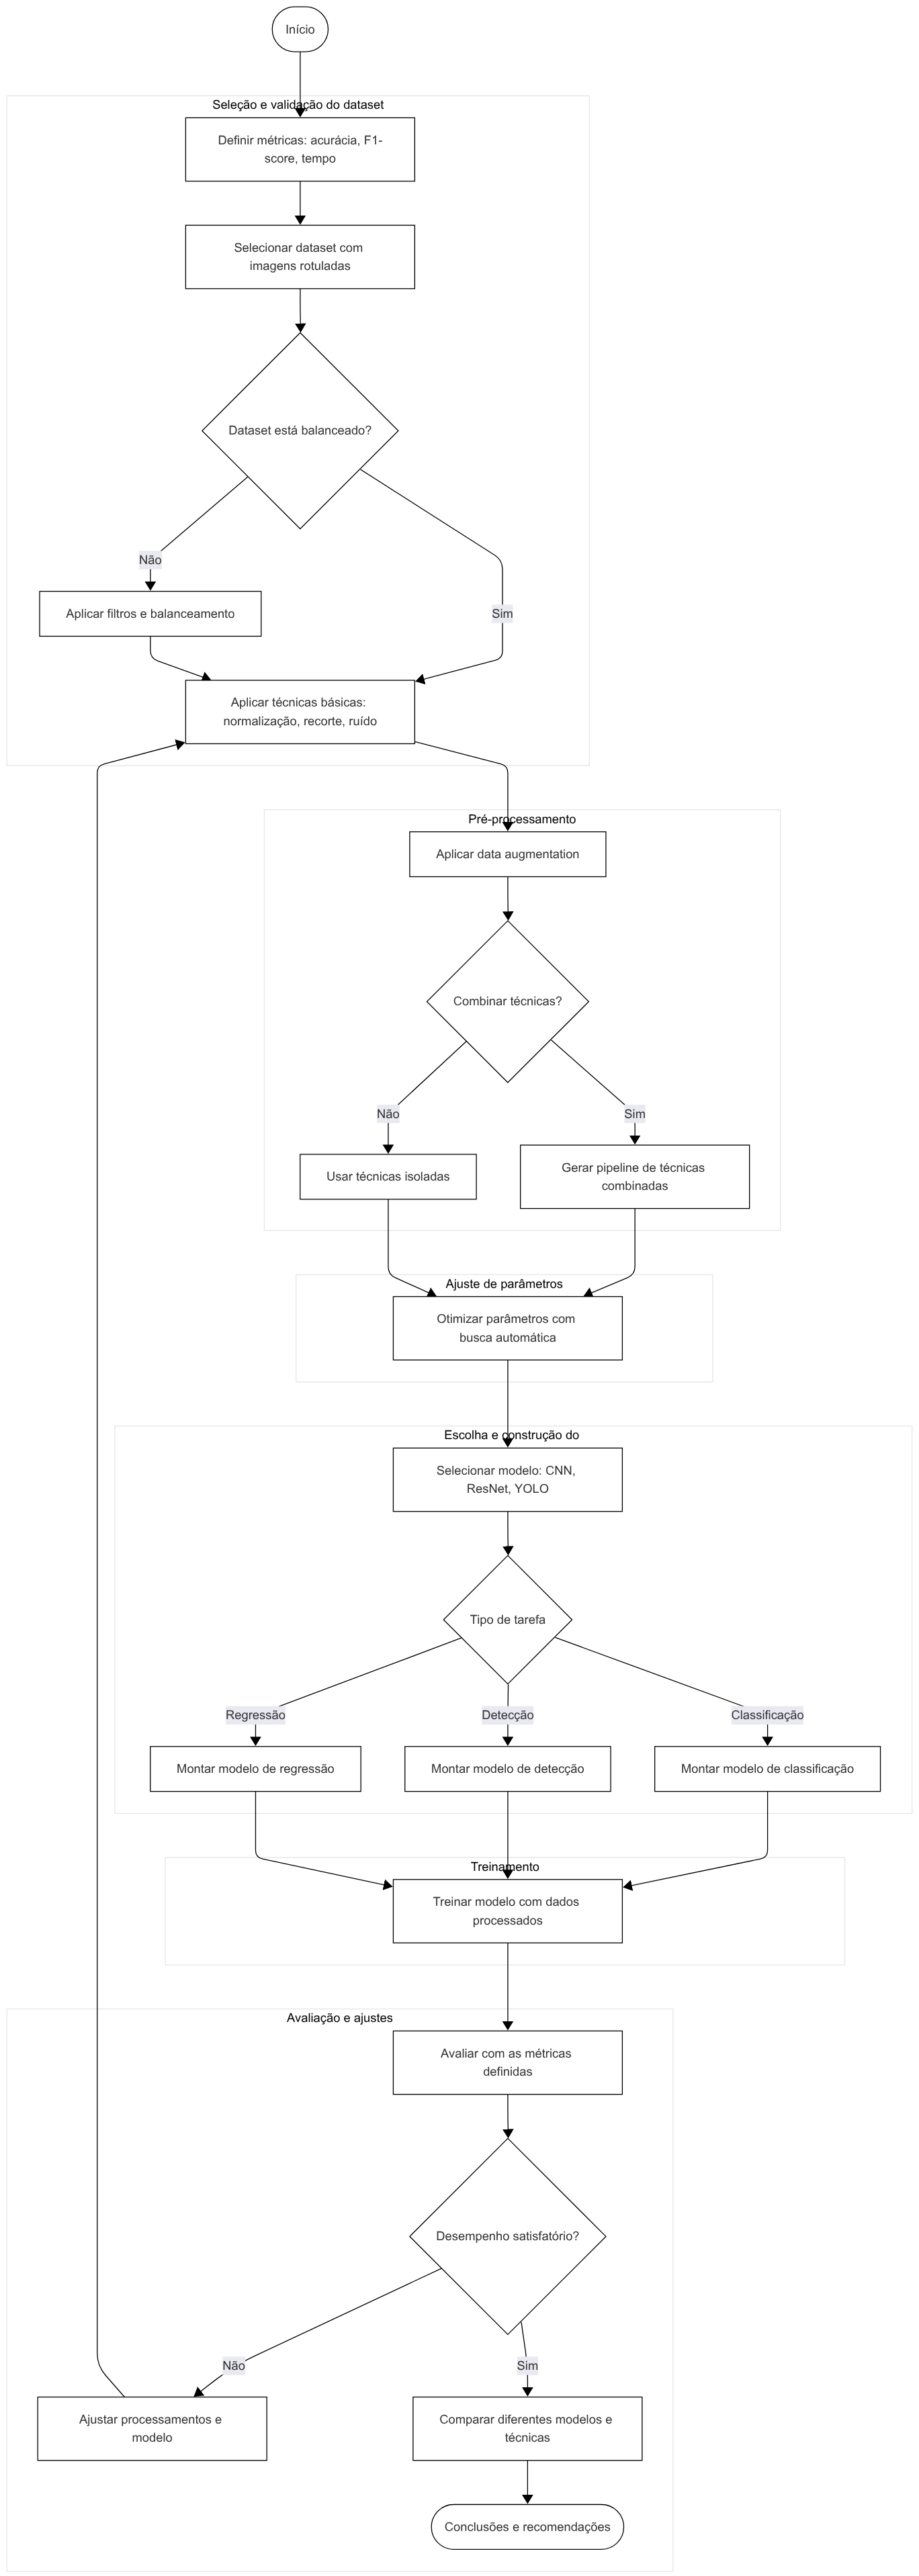
\includegraphics[width=0.5\textwidth]{img/metodologia.png}
    \fonte{Autor.}
\end{figure}

O fluxograma completo apresentado na Figura \ref{fig:fluxograma_metodologia} fornece uma visão macro de todas as etapas envolvidas na metodologia. Para facilitar a compreensão do fluxo e das inter-relações entre as fases, a Figura \ref{fig:fluxograma_geral} apresenta o fluxograma geral, que integra todos os fluxogramas menores das etapas subsequentes.

\begin{figure}[H]
    \centering
    \caption{\label{fig:fluxograma_geral}Fluxograma geral da metodologia, integrando todas as etapas principais}
    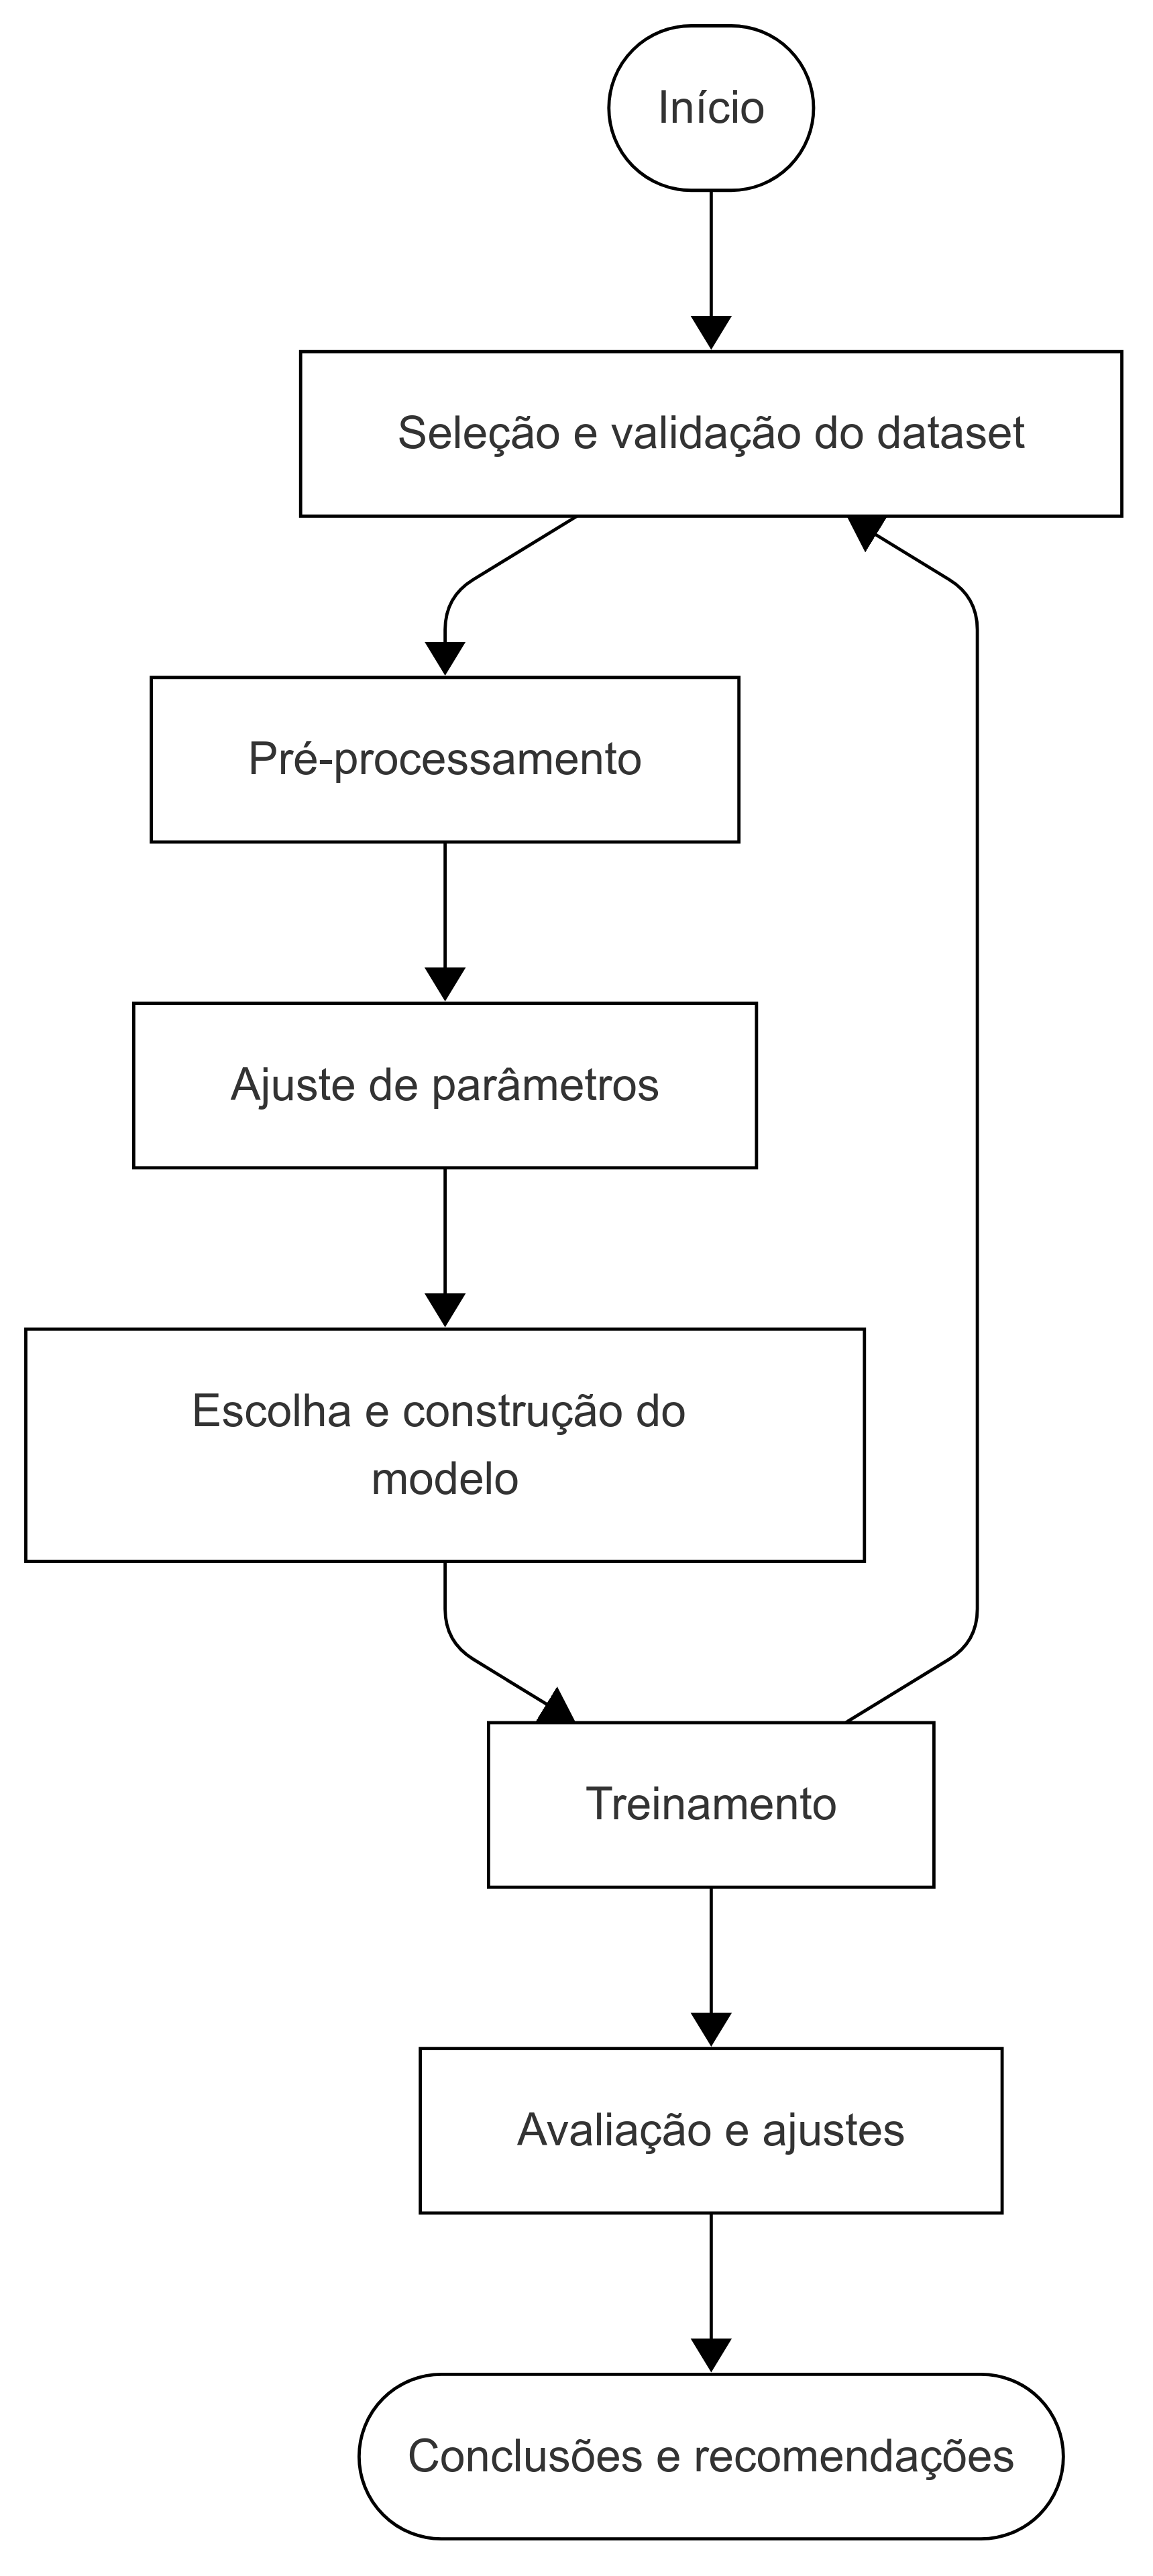
\includegraphics[width=0.5\textwidth]{img/metodologia - geral.png}
    \fonte{Autor.}
\end{figure}

O fluxograma da metodologia, apresentado na Figura \ref{fig:fluxograma_metodologia}, revela uma arquitetura robusta e pensada para a otimização de processamentos de imagens. Um dos pilares desta estrutura é a natureza iterativa do processo, evidenciada pelos ciclos de "Avaliação e ajustes" que retroalimentam as fases de "Pré-processamento" e "Escolha e construção do modelo". Essa recursividade é crucial, pois permite um refinamento contínuo das técnicas e parâmetros, adaptando-se aos resultados obtidos a cada iteração. A organização em módulos distintos, como "Seleção e validação do dataset", "Pré-processamento", "Ajuste de parâmetros", "Escolha e construção do modelo", "Treinamento" e "Avaliação e ajustes", é outra característica positiva, facilitando a depuração e o aprimoramento localizado de cada componente da metodologia. Essa modularidade assegura que, em caso de falhas ou resultados subótimos, a origem do problema possa ser isolada e corrigida eficientemente, sem comprometer a integridade do sistema como um todo.

A seguir, cada uma das principais fases do processo será detalhada em seções específicas, abordando desde a definição das métricas e preparação dos dados até as estratégias de aprimoramento e avaliação final dos resultados.

\section{Início e Definição de Métricas}

Esta seção aborda o ponto de partida da metodologia, incluindo a inicialização do ambiente e a definição das métricas que serão utilizadas para avaliar o desempenho ao longo de todo o processo.

\subsection{Início}
O bloco "Início" demarca o ponto de partida formal da execução desta metodologia. Sua função primordial é a de inicializar o ambiente computacional e todos os recursos necessários, garantindo que as ferramentas de software, as bibliotecas de programação estejam devidamente configuradas e acessíveis. A expectativa é que, ao transitar por este ponto, o sistema esteja preparado para as operações subsequentes de definição de métricas, coleta, tratamento e processamento de dados. A presença deste bloco, embora aparentemente trivial, é crucial para a organização lógica do fluxo de trabalho, servindo como um marco zero que assegura a rastreabilidade e a replicabilidade do experimento.

A dificuldade inerente a esta etapa é, em geral, baixa, confinando-se principalmente à fase de setup inicial do projeto. No cenário de um erro, como a falha na inicialização de bibliotecas ou na alocação de recursos, a ação corretiva imediata seria a verificação das dependências de software, a compatibilidade de versões e a adequação do hardware (por exemplo, disponibilidade de GPUs para aceleração de treinamento). A avaliação do sucesso é intrínseca à própria continuidade do fluxograma: uma transição fluida para o próximo estágio é o indicador de que o "Início" foi bem-sucedido. Este bloco, portanto, alinha-se diretamente ao objetivo geral de desenvolver uma metodologia capaz de comparar, selecionar, combinar e aprimorar técnicas de processamento de imagem, pois estabelece as bases operacionais para todas as etapas subsequentes. Sem essa formalização inicial, a execução do projeto careceria de um ponto de partida definido, comprometendo a sistematicidade proposta.

\section{Seleção e Validação do Dataset}

Esta seção detalha o processo de seleção, validação e preparação dos dados que servirão como base para todo o desenvolvimento da metodologia. O fluxograma específico desta etapa é apresentado na Figura \ref{fig:fluxograma_selecao_dataset}, permitindo visualizar de forma clara o caminho percorrido desde a definição das métricas até o balanceamento dos dados.

\begin{figure}[H]
    \centering
    \caption{\label{fig:fluxograma_selecao_dataset}Fluxograma da etapa de seleção e validação do dataset}
    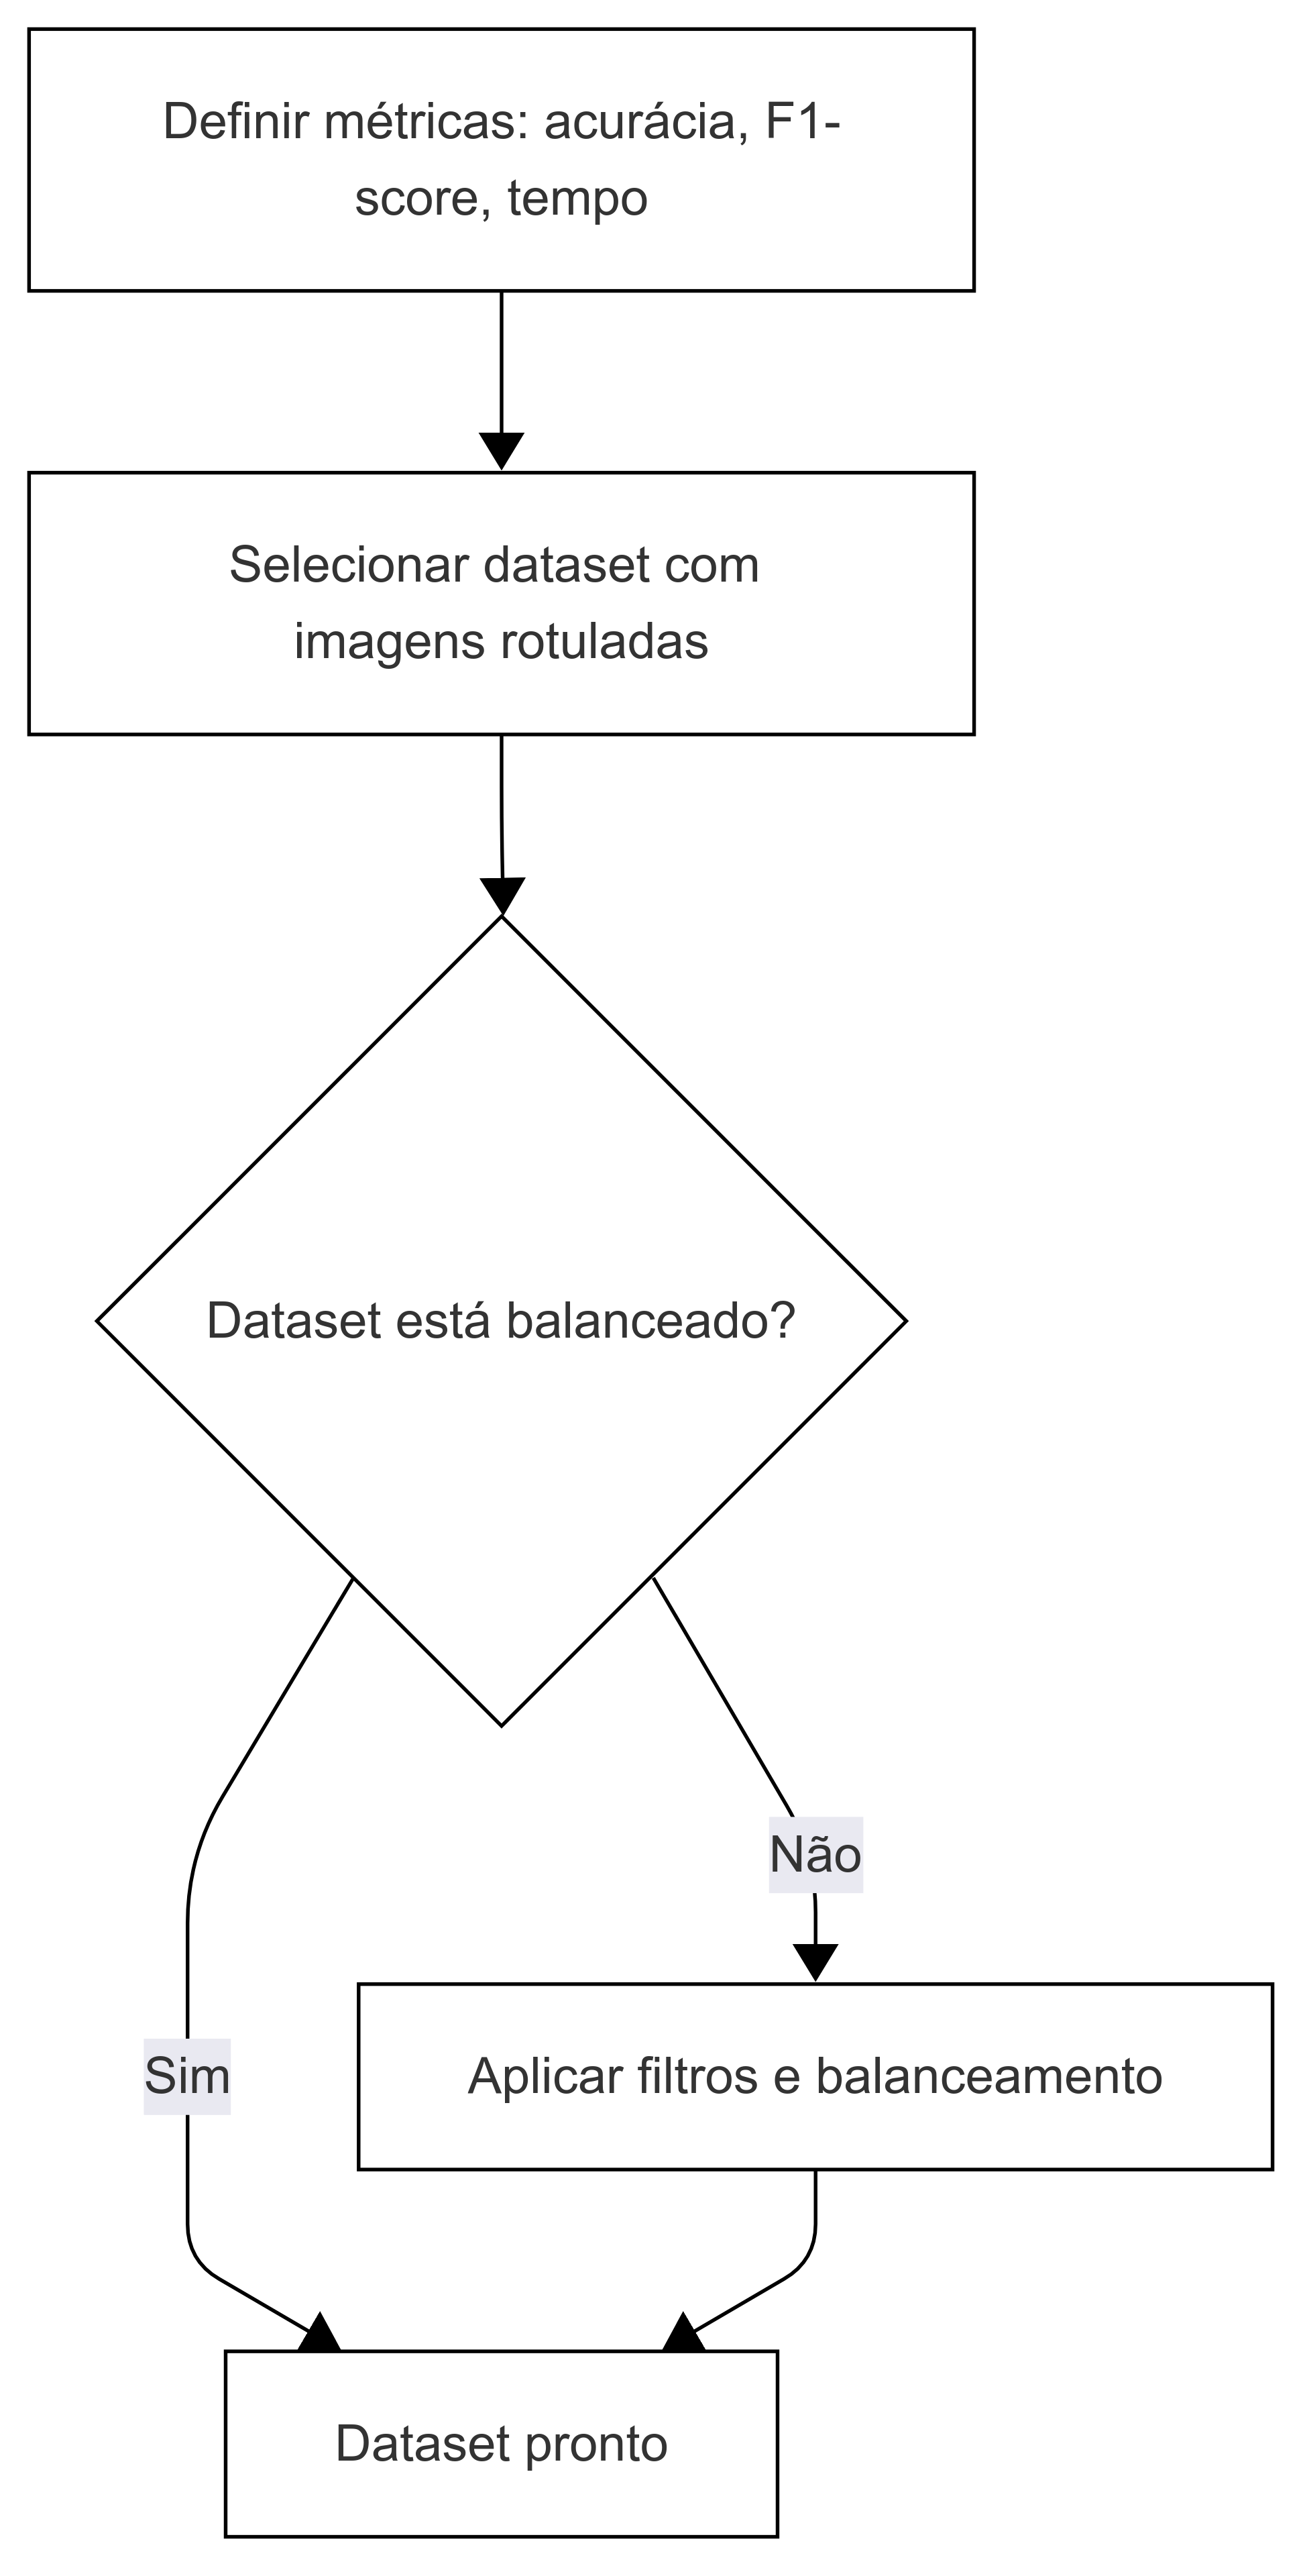
\includegraphics[width=0.6\textwidth]{img/metodologia - 1 - seleção e validação do dataset.png}
    \fonte{Autor.}
\end{figure}

\subsection{Definir métricas: acurácia, F1-score, tempo}
O bloco "Definir métricas: acurácia, F1-score, tempo" é fundamental para estabelecer os critérios objetivos de avaliação que irão nortear todo o processo de otimização da metodologia. A expectativa é que, nesta fase inicial, sejam claramente especificadas as métricas que serão utilizadas para medir o sucesso das diferentes combinações de técnicas de processamento de imagem e arquiteturas de modelos. A definição prévia dessas métricas é crucial porque elas servirão como bússola para todas as decisões subsequentes, desde a seleção de técnicas de pré-processamento até a escolha final dos modelos mais eficazes.

As três métricas principais definidas - acurácia, F1-score e tempo de processamento - foram selecionadas por fornecerem uma visão abrangente do desempenho do sistema. A acurácia oferece uma medida geral de correção das predições, o F1-score é especialmente valioso para datasets desbalanceados por combinar precisão e recall de forma harmônica, e o tempo de processamento é essencial para aplicações práticas onde a eficiência computacional é crítica, como na inspeção automatizada de linhas de transmissão.

A dificuldade de execução desta etapa é baixa, sendo principalmente conceitual e de planejamento. Um erro comum seria a definição de métricas inadequadas para o tipo de problema ou a omissão de métricas relevantes para a aplicação específica. Se as métricas inicialmente definidas se mostrarem insuficientes durante o desenvolvimento, a ação corretiva seria a revisão e refinamento dos critérios de avaliação, sempre mantendo a coerência com os objetivos do estudo. A avaliação do sucesso desta etapa é confirmada pela clareza e adequação das métricas definidas para o contexto do problema de detecção de falhas em isoladores. Este bloco é fundamental para o objetivo geral da metodologia, pois estabelece as bases quantitativas para todas as comparações e seleções que serão realizadas ao longo do processo.

\subsection{Selecionar dataset com imagens rotuladas}
A etapa de "Selecionar dataset com imagens rotuladas" é uma das mais críticas e de maior impacto sobre a qualidade e a confiabilidade dos resultados. A expectativa é que, nesta fase, seja escolhido um conjunto de dados adequado que contenha imagens de cadeias de isoladores com anotações precisas indicando a presença ou ausência de falhas. O dataset deve apresentar diversidade suficiente em termos de condições de iluminação, ângulos de captura, tipos de isoladores e variações de falhas para garantir que os modelos desenvolvidos tenham boa capacidade de generalização.

Esta etapa é fundamental porque a qualidade, quantidade e diversidade dos dados impactam diretamente o desempenho e a capacidade de generalização dos modelos de aprendizado de máquina. Sem dados adequados e bem rotulados, qualquer processamento subsequente será comprometido. Como mencionado por \citeonline{Shorten2019}, a robustez de um modelo depende intrinsecamente da riqueza de seu conjunto de treinamento.

A dificuldade de execução pode ser consideravelmente alta devido à escassez de datasets públicos específicos para detecção de falhas em isoladores e à necessidade de anotação manual precisa. Se o dataset selecionado se mostrar inadequado, as ações corretivas podem incluir a busca por datasets alternativos, a combinação de múltiplos datasets ou a criação de um dataset próprio através de coleta e anotação manual de imagens.

\subsection{Dataset está balanceado?}
O bloco de decisão "Dataset está balanceado?" é um ponto crítico de validação que verifica se as classes de interesse (isoladores com falha e sem falha) estão adequadamente representadas no dataset selecionado. A expectativa é que esta verificação identifique possíveis desbalanceamentos que poderiam comprometer o treinamento dos modelos, levando a vieses onde o modelo favorece a classe majoritária.

O balanceamento é especialmente importante em problemas de detecção de falhas, onde frequentemente há muito mais amostras de isoladores saudáveis do que defeituosos. Essa assimetria, conforme \citeonline{He2009}, pode levar a modelos enviesados que apresentam alta acurácia geral, mas baixa capacidade de detectar as falhas, que são justamente o objetivo principal do sistema.

A dificuldade desta etapa é baixa, envolvendo principalmente análise estatística das distribuições das classes. Se o dataset estiver desbalanceado, o fluxo direciona para a aplicação de filtros e balanceamento; caso contrário, prossegue diretamente para o pré-processamento.

\subsection{Aplicar filtros e balanceamento}
O bloco "Aplicar filtros e balanceamento" é executado quando o dataset se mostra desbalanceado, implementando estratégias para corrigir a distribuição desigual entre as classes. A expectativa é que esta etapa aplique técnicas como reamostragem (sobreamostragem da classe minoritária através de duplicação ou técnicas como SMOTE, ou subamostragem da classe majoritária), aplicação de pesos diferenciados nas funções de perda, ou técnicas de data augmentation focadas na classe minoritária.

Esta etapa é crucial porque o desbalanceamento pode significativamente comprometer a capacidade do modelo de detectar falhas, que são tipicamente a classe minoritária mas a mais importante do ponto de vista prático. A aplicação de filtros também pode envolver a remoção de amostras de baixa qualidade ou outliers que poderiam prejudicar o treinamento.

A dificuldade de execução pode ser de média a alta, dependendo do grau de desbalanceamento e das técnicas escolhidas. Se as técnicas de balanceamento não forem eficazes, as ações corretivas podem incluir a exploração de métodos alternativos de balanceamento, a revisão dos critérios de qualidade das amostras, ou a busca por dados adicionais para a classe minoritária.

\section{Pré-processamento}

Esta seção detalha as etapas de processamento de imagens que visam otimizar os dados de entrada para maximizar o desempenho dos modelos de rede neural. O fluxograma da Figura \ref{fig:fluxograma_preprocessamento} ilustra as decisões e operações realizadas nesta fase.

\begin{figure}[H]
    \centering
    \caption{\label{fig:fluxograma_preprocessamento}Fluxograma da etapa de pré-processamento}
    \includegraphics[width=0.85\textwidth]{img/metodologia - 2 - pré-processamento.png}
    \fonte{Autor.}
\end{figure}

\subsection{Aplicar técnicas básicas: normalização, recorte, ruído}
O bloco "Aplicar técnicas básicas: normalização, recorte, ruído" é uma fase fundamental onde as imagens são submetidas a processamentos essenciais para maximizar a eficácia dos modelos de rede neural. A expectativa é que esta etapa envolva a aplicação de técnicas fundamentais como a normalização (padronização dos valores de pixels para escalas como [0,1] ou Z-score) \cite{Sharma2024}, o redimensionamento e recorte (ajustando imagens para as dimensões de entrada do modelo e extraindo regiões de interesse) \cite{Sharma2024}, e a redução de ruído (eliminando interferências com filtros como mediana ou filtros gaussianos) \cite{Sharma2024}.

Essas operações são cruciais porque, como afirmado por \citeonline{Sharma2024}, elas "melhoram a qualidade das imagens, mas também garantem que os modelos sejam mais robustos e capazes de generalizar em diferentes condições". A normalização é especialmente importante para garantir convergência estável durante o treinamento, enquanto o recorte adequado pode focar a atenção do modelo nas regiões mais relevantes da imagem.

A dificuldade de execução é geralmente baixa a média, sendo técnicas bem estabelecidas na literatura. Se o desempenho do modelo piorar após a aplicação dessas técnicas básicas, a ação corretiva seria revisar os parâmetros aplicados ou a ordem de aplicação das técnicas, buscando um equilíbrio ideal.

\subsection{Aplicar data augmentation}
O bloco "Aplicar data augmentation" tem como objetivo expandir artificialmente o dataset através de transformações que preservam as características essenciais das imagens mas introduzem variabilidade que pode melhorar a capacidade de generalização do modelo. A expectativa é que esta etapa aplique transformações como rotações, espelhamentos, ajustes de brilho e contraste, mudanças de escala, e translações, criando variações das imagens originais que simulam diferentes condições de captura.

O data augmentation é especialmente valioso quando o dataset é limitado ou desbalanceado, pois pode artificialmente aumentar o número de amostras disponíveis para treinamento. Como mencionado por \citeonline{Shorten2019}, técnicas de aumento de dados são fundamentais para melhorar a robustez dos modelos de aprendizado profundo.

A dificuldade de execução é baixa a média, mas requer cuidado para não aplicar transformações que alterem características importantes para a detecção de falhas. Se o data augmentation degradar o desempenho, as ações corretivas incluem revisar os tipos e intensidades das transformações aplicadas.

\subsection{Combinar técnicas?}
O bloco de decisão "Combinar técnicas?" determina se múltiplas técnicas de processamento serão aplicadas em sequência para criar um pipeline de processamento mais sofisticado. Esta decisão é estratégica, pois combinar técnicas pode resultar em melhorias sinérgicas, mas também pode introduzir complexidade desnecessária ou até mesmo degradação da qualidade da imagem.

A expectativa é que esta decisão seja baseada nos resultados preliminares das técnicas aplicadas individualmente e no conhecimento de domínio sobre quais combinações podem ser benéficas. Por exemplo, aplicar redução de ruído seguida por aumento de nitidez pode resultar em imagens mais adequadas para detecção de defeitos.

A dificuldade desta etapa é baixa, sendo principalmente uma decisão estratégica. Se a decisão for por combinar técnicas, o fluxo segue para a geração de pipelines combinados. Caso contrário, utiliza as técnicas de forma isolada.

\subsection{Gerar pipeline de técnicas combinadas}
O bloco "Gerar pipeline de técnicas combinadas" é executado quando se decide explorar a sinergia entre diferentes técnicas de processamento de imagem. A expectativa é que esta etapa crie sequências estratégicas de processamentos, onde a saída de uma técnica serve como entrada para a próxima, buscando um efeito cumulativo que transcenda o impacto de cada técnica isolada.

Por exemplo, um pipeline pode consistir em: normalização → redução de ruído → ajuste de contraste → aumento de nitidez. A ordem das operações é crucial, pois diferentes sequências podem produzir resultados significativamente diferentes. O propósito é explorar o potencial de melhoria que reside na interação entre diferentes processamentos.

A dificuldade de execução pode ser de média a alta, principalmente devido à explosão combinatória de possibilidades e à necessidade de identificar as sequências mais eficazes. Um erro comum é criar combinações que introduzem artefatos ou degradam a imagem. Se as combinações não trouxerem melhorias, as ações corretivas incluem explorar diferentes ordens de aplicação ou revisar a seleção de técnicas.

\subsection{Usar técnicas isoladas}
O bloco "Usar técnicas isoladas" é executado quando se decide não combinar múltiplas técnicas, optando por aplicar e avaliar cada processamento de forma independente. Esta abordagem é mais simples e permite uma avaliação clara do impacto individual de cada técnica, facilitando a identificação de quais processamentos são mais eficazes para o problema específico.

A expectativa é que cada técnica seja aplicada, avaliada e comparada individualmente, criando um benchmark claro do desempenho de cada abordagem. Esta estratégia é especialmente útil nas fases iniciais do desenvolvimento, quando se busca entender o impacto individual de cada processamento.

A dificuldade de execução é baixa, sendo uma abordagem mais direta. A avaliação do sucesso é feita comparando o desempenho do modelo com cada técnica aplicada individualmente versus o desempenho baseline sem processamento.

\section{Ajuste de Parâmetros}

Esta seção detalha o processo de otimização automática dos parâmetros das técnicas de processamento de imagem. O fluxograma da Figura \ref{fig:fluxograma_ajuste_parametros} apresenta o fluxo de etapa única de ajuste automático dos parâmetros.

\begin{figure}[H]
    \centering
    \caption{\label{fig:fluxograma_ajuste_parametros}Fluxograma da etapa de ajuste de parâmetros}
    \includegraphics[width=0.5\textwidth]{img/metodologia - 3 - ajustes de parâmetros.png}
    \fonte{Autor.}
\end{figure}

\subsection{Otimizar parâmetros com busca automática}
O bloco "Otimizar parâmetros com busca automática" representa um avanço significativo na eficiência da metodologia, substituindo a tediosa e muitas vezes inviável otimização manual. A expectativa é que, nesta fase, algoritmos de otimização automatizada sejam empregados para encontrar os valores ideais para os parâmetros das técnicas de processamento de imagem que estão sendo testadas. Isso pode incluir, por exemplo, a intensidade de um filtro de desfoque, o limiar de um ajuste de contraste, os parâmetros de técnicas de redução de ruído, ou os fatores de data augmentation.

O propósito fundamental deste bloco é otimizar os resultados dos processamentos sem exigir extensa intervenção manual, como destacado na proposta da metodologia. A automação não apenas acelera o processo, mas também tem o potencial de descobrir configurações de parâmetros que seriam difíceis de identificar heuristicamente. Métodos como busca em grade (grid search), busca aleatória (random search), otimização Bayesiana, algoritmos genéticos, ou otimização por enxame de partículas podem ser empregados dependendo da complexidade do espaço de parâmetros.

A dificuldade de execução pode ser alta, pois envolve a seleção e implementação de algoritmos de otimização apropriados e a definição de um espaço de busca adequado para os parâmetros. Um erro comum é a convergência para ótimos locais em vez do ótimo global, ou um tempo computacional proibitivo para a busca. Se o ajuste automático não encontrar parâmetros que resultem em melhorias significativas, as ações corretivas podem incluir: a modificação do algoritmo de otimização, a redefinição das faixas de valores para os parâmetros, ou a incorporação de critérios de parada mais sofisticados.

A avaliação do sucesso é diretamente quantitativa: a melhoria mensurável nas métricas de desempenho do modelo de rede neural após a aplicação dos parâmetros otimizados automaticamente indica que o processo foi bem-sucedido. Este bloco está diretamente ligado ao objetivo específico de criar um método de ajuste automático de parâmetros dos processamentos de imagem, sendo um pilar central para o aprimoramento contínuo e eficiente das técnicas.

\section{Escolha e Construção do Modelo}

Esta seção detalha o processo de seleção e configuração das arquiteturas de redes neurais que serão utilizadas para avaliar a eficácia das técnicas de processamento de imagem. O fluxograma da Figura \ref{fig:fluxograma_escolha_modelo} ilustra as decisões envolvidas na escolha e montagem do modelo.

\begin{figure}[H]
    \centering
    \caption{\label{fig:fluxograma_escolha_modelo}Fluxograma da etapa de escolha e construção do modelo}
    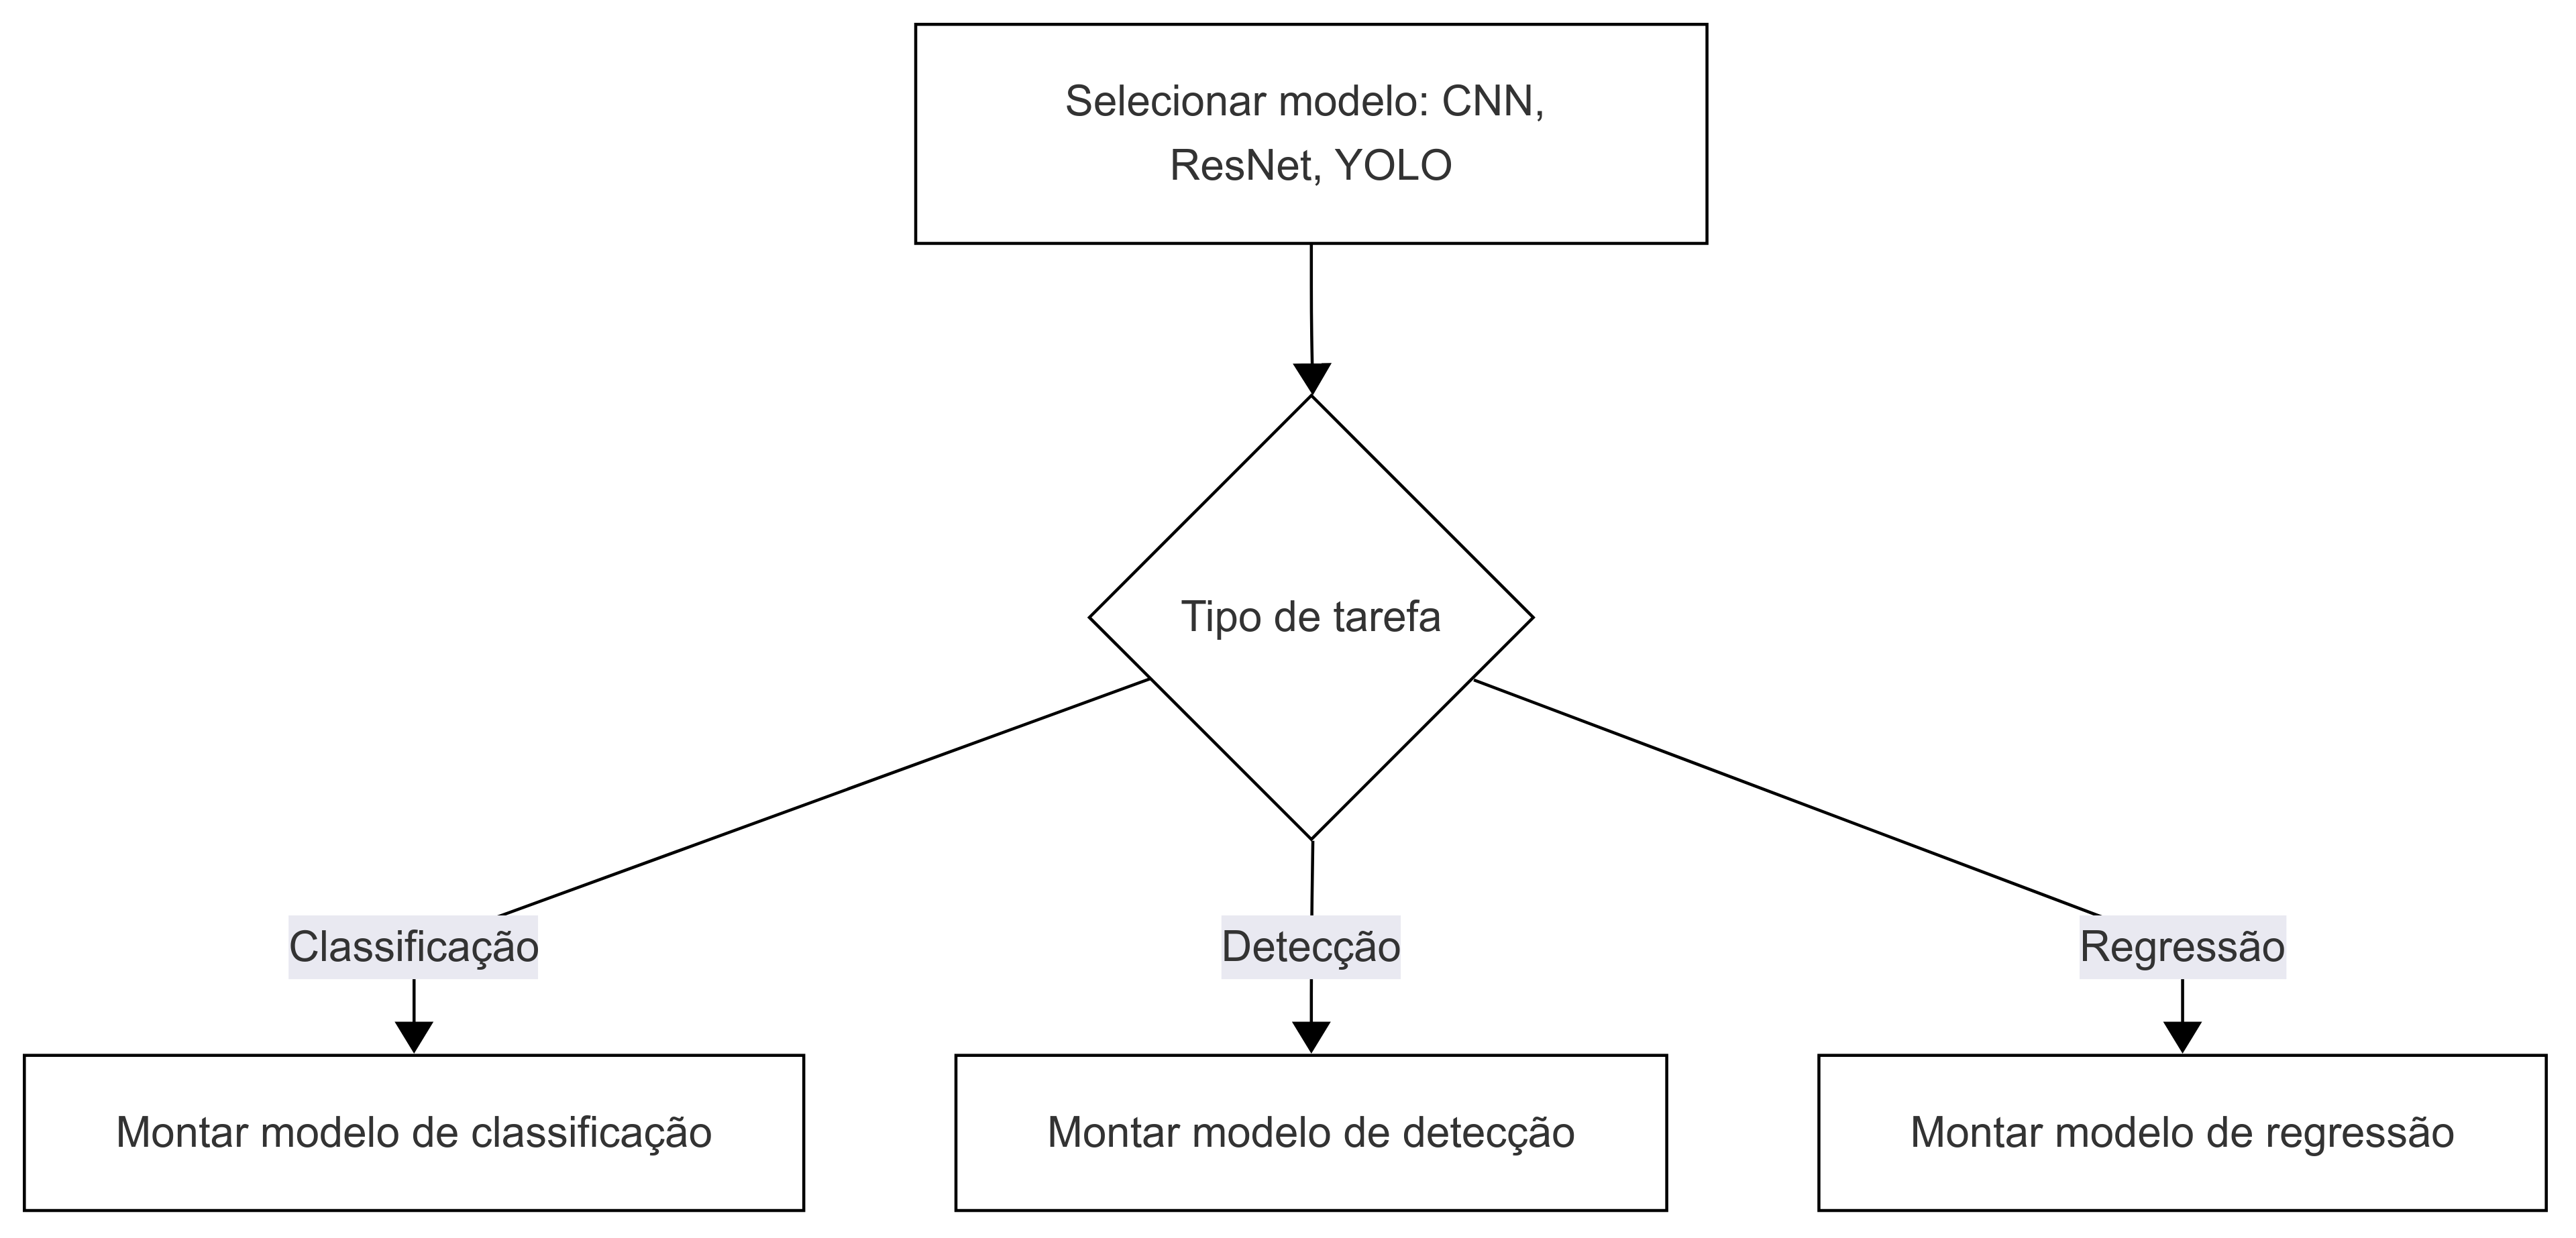
\includegraphics[width=1\textwidth]{img/metodologia - 4 - escolha e construção do modelo.png}
    \fonte{Autor.}
\end{figure}

\subsection{Selecionar modelo: CNN, ResNet, YOLO}
O bloco "Selecionar modelo: CNN, ResNet, YOLO" representa um ponto estratégico na metodologia onde é definida a arquitetura de rede neural que será utilizada para avaliar o impacto das técnicas de processamento de imagem. A expectativa é que esta seleção seja baseada na natureza específica da tarefa (classificação, detecção, ou regressão) e nas características do problema de detecção de falhas em isoladores.

As opções apresentadas cobrem diferentes abordagens: CNNs convencionais para tarefas de classificação básica, ResNet para problemas que requerem redes mais profundas, e YOLO para tarefas de detecção de objetos em tempo real. A escolha da arquitetura é crucial pois, como apontado na literatura, diferentes tipos de redes neurais possuem princípios de funcionamento e aplicações práticas distintas.

A dificuldade de execução deste bloco é relativamente baixa, sendo principalmente uma decisão estratégica baseada nos requisitos do problema. No entanto, uma escolha inadequada pode comprometer significativamente os resultados subsequentes. Se a arquitetura selecionada não apresentar o desempenho esperado, a ação corretiva seria a reavaliação da escolha, considerando as características específicas dos dados e os objetivos da aplicação.

\subsection{Tipo de tarefa}
O bloco de decisão "Tipo de tarefa" é fundamental para direcionar a configuração específica do modelo selecionado. Esta decisão determina como a arquitetura escolhida será configurada e treinada, influenciando aspectos como a função de perda, as métricas de avaliação, e a estrutura das camadas finais da rede.

As três opções principais são: classificação (determinar se um isolador possui falha ou não), detecção (localizar e classificar falhas nas imagens), e regressão (predizer valores contínuos relacionados ao grau de degradação). Cada tipo de tarefa requer configurações específicas do modelo e métricas de avaliação apropriadas.

A dificuldade desta etapa é baixa, sendo uma decisão conceitual baseada nos objetivos específicos do estudo. A escolha correta é essencial para que o modelo seja apropriadamente configurado para o problema em questão.

\subsection{Montar modelo de classificação}
O bloco "Montar modelo de classificação" é executado quando a tarefa escolhida é classificação. A expectativa é que nesta etapa seja configurada uma rede neural para classificar imagens de isoladores em categorias discretas (por exemplo, "com falha" vs "sem falha", ou múltiplas classes de diferentes tipos de falhas).

A configuração inclui a definição das camadas finais da rede com um número de neurônios correspondente ao número de classes, a seleção de funções de ativação apropriadas (como softmax para classificação multiclasse), e a escolha de funções de perda adequadas (como cross-entropy). Também envolve a definição das métricas de avaliação relevantes como acurácia, precisão, recall e F1-score.

A dificuldade de execução é média, requerendo conhecimento técnico sobre arquiteturas de redes neurais para classificação. Se o modelo não apresentar desempenho satisfatório, as ações corretivas podem incluir ajustes na arquitetura, modificação dos hiperparâmetros, ou revisão do pré-processamento dos dados.

\subsection{Montar modelo de detecção}
O bloco "Montar modelo de detecção" é executado quando a tarefa escolhida é detecção de objetos. A expectativa é que seja configurado um modelo capaz não apenas de classificar a presença de falhas, mas também de localizar espacialmente essas falhas nas imagens, fornecendo coordenadas de bounding boxes ou máscaras de segmentação.

Esta configuração é mais complexa, envolvendo arquiteturas especializadas como YOLO, R-CNN, ou outras redes de detecção. Inclui a definição de hiperparâmetros, configuração de múltiplas escalas, e o balanceamento entre precisão de localização e classificação. As métricas de avaliação incluem mAP (mean Average Precision) e IoU (Intersection over Union).

A dificuldade de execução é alta, devido à complexidade das arquiteturas de detecção e à necessidade de dados rotulados com informações de localização. Se o desempenho não for satisfatório, as ações corretivas podem incluir ajustes nos hiperparâmetros, modificação dos thresholds de confiança, ou revisão da estratégia de aumento de dados.

\subsection{Montar modelo de regressão}
O bloco "Montar modelo de regressão" é executado quando a tarefa escolhida é regressão. A expectativa é que seja configurado um modelo capaz de predizer valores contínuos relacionados ao estado dos isoladores, como grau de degradação, probabilidade de falha, ou índices de severidade.

A configuração inclui camadas finais com ativação linear ou outras funções apropriadas para saídas contínuas, seleção de funções de perda para regressão (como MSE ou MAE), e definição de métricas de avaliação como R², RMSE, ou MAE. Esta abordagem pode ser útil quando se deseja uma avaliação mais detalhada do estado dos isoladores.

A dificuldade de execução é média, similar à classificação mas com considerações específicas para saídas contínuas. Se o modelo não apresentar predições adequadas, as ações corretivas podem incluir normalização das variáveis de saída, ajustes na função de perda, ou modificação da arquitetura da rede.

\section{Treinamento}

Esta seção detalha o processo de treinamento dos modelos de rede neural utilizando os dados processados. O fluxograma da Figura \ref{fig:fluxograma_treinamento} apresenta o fluxo de atividades desta etapa.

\begin{figure}[H]
    \centering
    \caption{\label{fig:fluxograma_treinamento}Fluxograma da etapa de treinamento}
    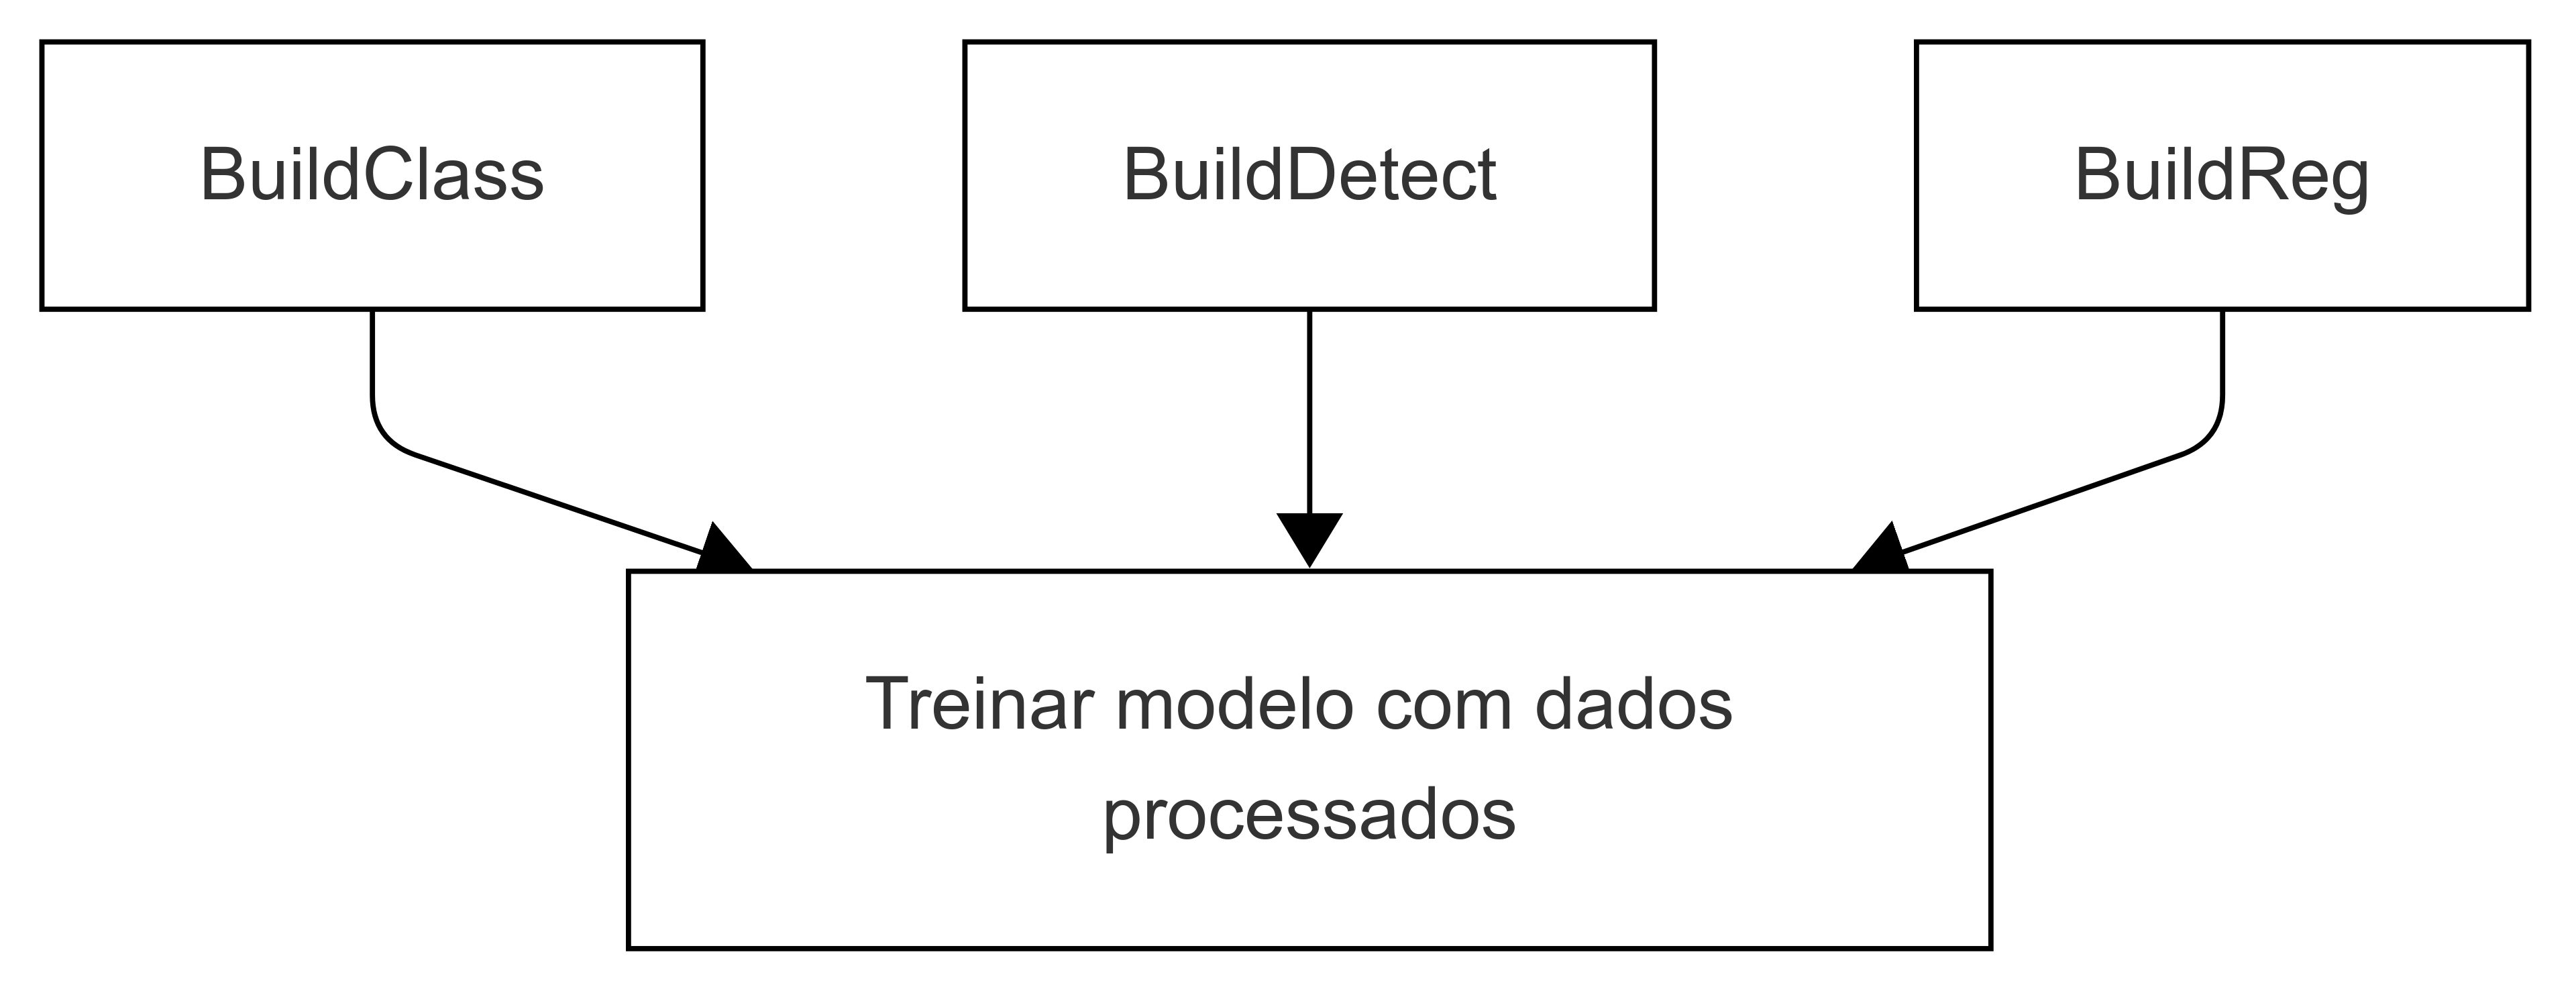
\includegraphics[width=0.85\textwidth]{img/metodologia - 5 - treinamento.png}
    \fonte{Autor.}
\end{figure}

\subsection{Treinar modelo com dados processados}
O bloco "Treinar modelo com dados processados" é o cerne do aprendizado e da adaptação do sistema. A expectativa é que, nesta fase, a arquitetura da rede neural previamente selecionada e configurada seja treinada utilizando os dados que passaram pelas etapas de processamento de imagem otimizadas. O propósito central é que o modelo aprenda a identificar e classificar as falhas nas imagens de isoladores, ajustando seus pesos e parâmetros de forma a minimizar a função de custo e otimizar as métricas de desempenho previamente definidas.

Como explicado em \citeonline{Braga2011}, o treinamento é onde o neurônio artificial aprende a associar entradas a saídas desejadas. A importância deste bloco é vital, pois os modelos de redes neurais não são apenas as ferramentas para a detecção de falhas, mas também os avaliadores do impacto dos diferentes processamentos de imagem aplicados nas etapas anteriores.

O processo de treinamento envolve a alimentação das imagens processadas através da rede neural, o cálculo do erro entre as predições e os rótulos verdadeiros, e a atualização dos pesos através de algoritmos de retropropagação. Durante esta etapa, é crucial monitorar métricas como a função de custo, acurácia de treinamento e validação para detectar possíveis problemas como overfitting ou underfitting.

A dificuldade de execução pode ser alta, dada a complexidade do treinamento de redes neurais. Desafios incluem a otimização de hiperparâmetros (como taxa de aprendizado, tamanho do batch, número de épocas), o gerenciamento de recursos computacionais (tempo de processamento, memória de GPU) e a mitigação do sobreajuste. Se o modelo não convergir, apresentar baixo desempenho ou sobreajuste, as ações corretivas podem envolver: a modificação dos hiperparâmetros do treinamento, a escolha de otimizadores mais adequados (como Adam ou RMSProp), a aplicação de técnicas de regularização (como dropout), ou a revisão da própria arquitetura da rede neural.

A diminuição progressiva da função de custo durante o treinamento e, crucialmente, o aumento das métricas de desempenho (acurácia, F1-score, tempo de processamento) nos conjuntos de validação e teste, indicam que o modelo está aprendendo de forma eficaz. Este bloco alinha-se diretamente ao objetivo de construir modelos de redes neurais destinados à avaliação do desempenho das técnicas de processamento de imagem, pois é através do treinamento que esses modelos adquirem a capacidade de realizar tal avaliação com precisão.

\section{Avaliação e Ajustes}

Esta seção detalha o processo de avaliação dos resultados obtidos e os mecanismos de ajuste que permitem a melhoria iterativa da metodologia. O fluxograma da Figura \ref{fig:fluxograma_avaliacao} ilustra o ciclo de avaliação e ajustes.

\begin{figure}[H]
    \centering
    \caption{\label{fig:fluxograma_avaliacao}Fluxograma da etapa de avaliação e ajustes}
    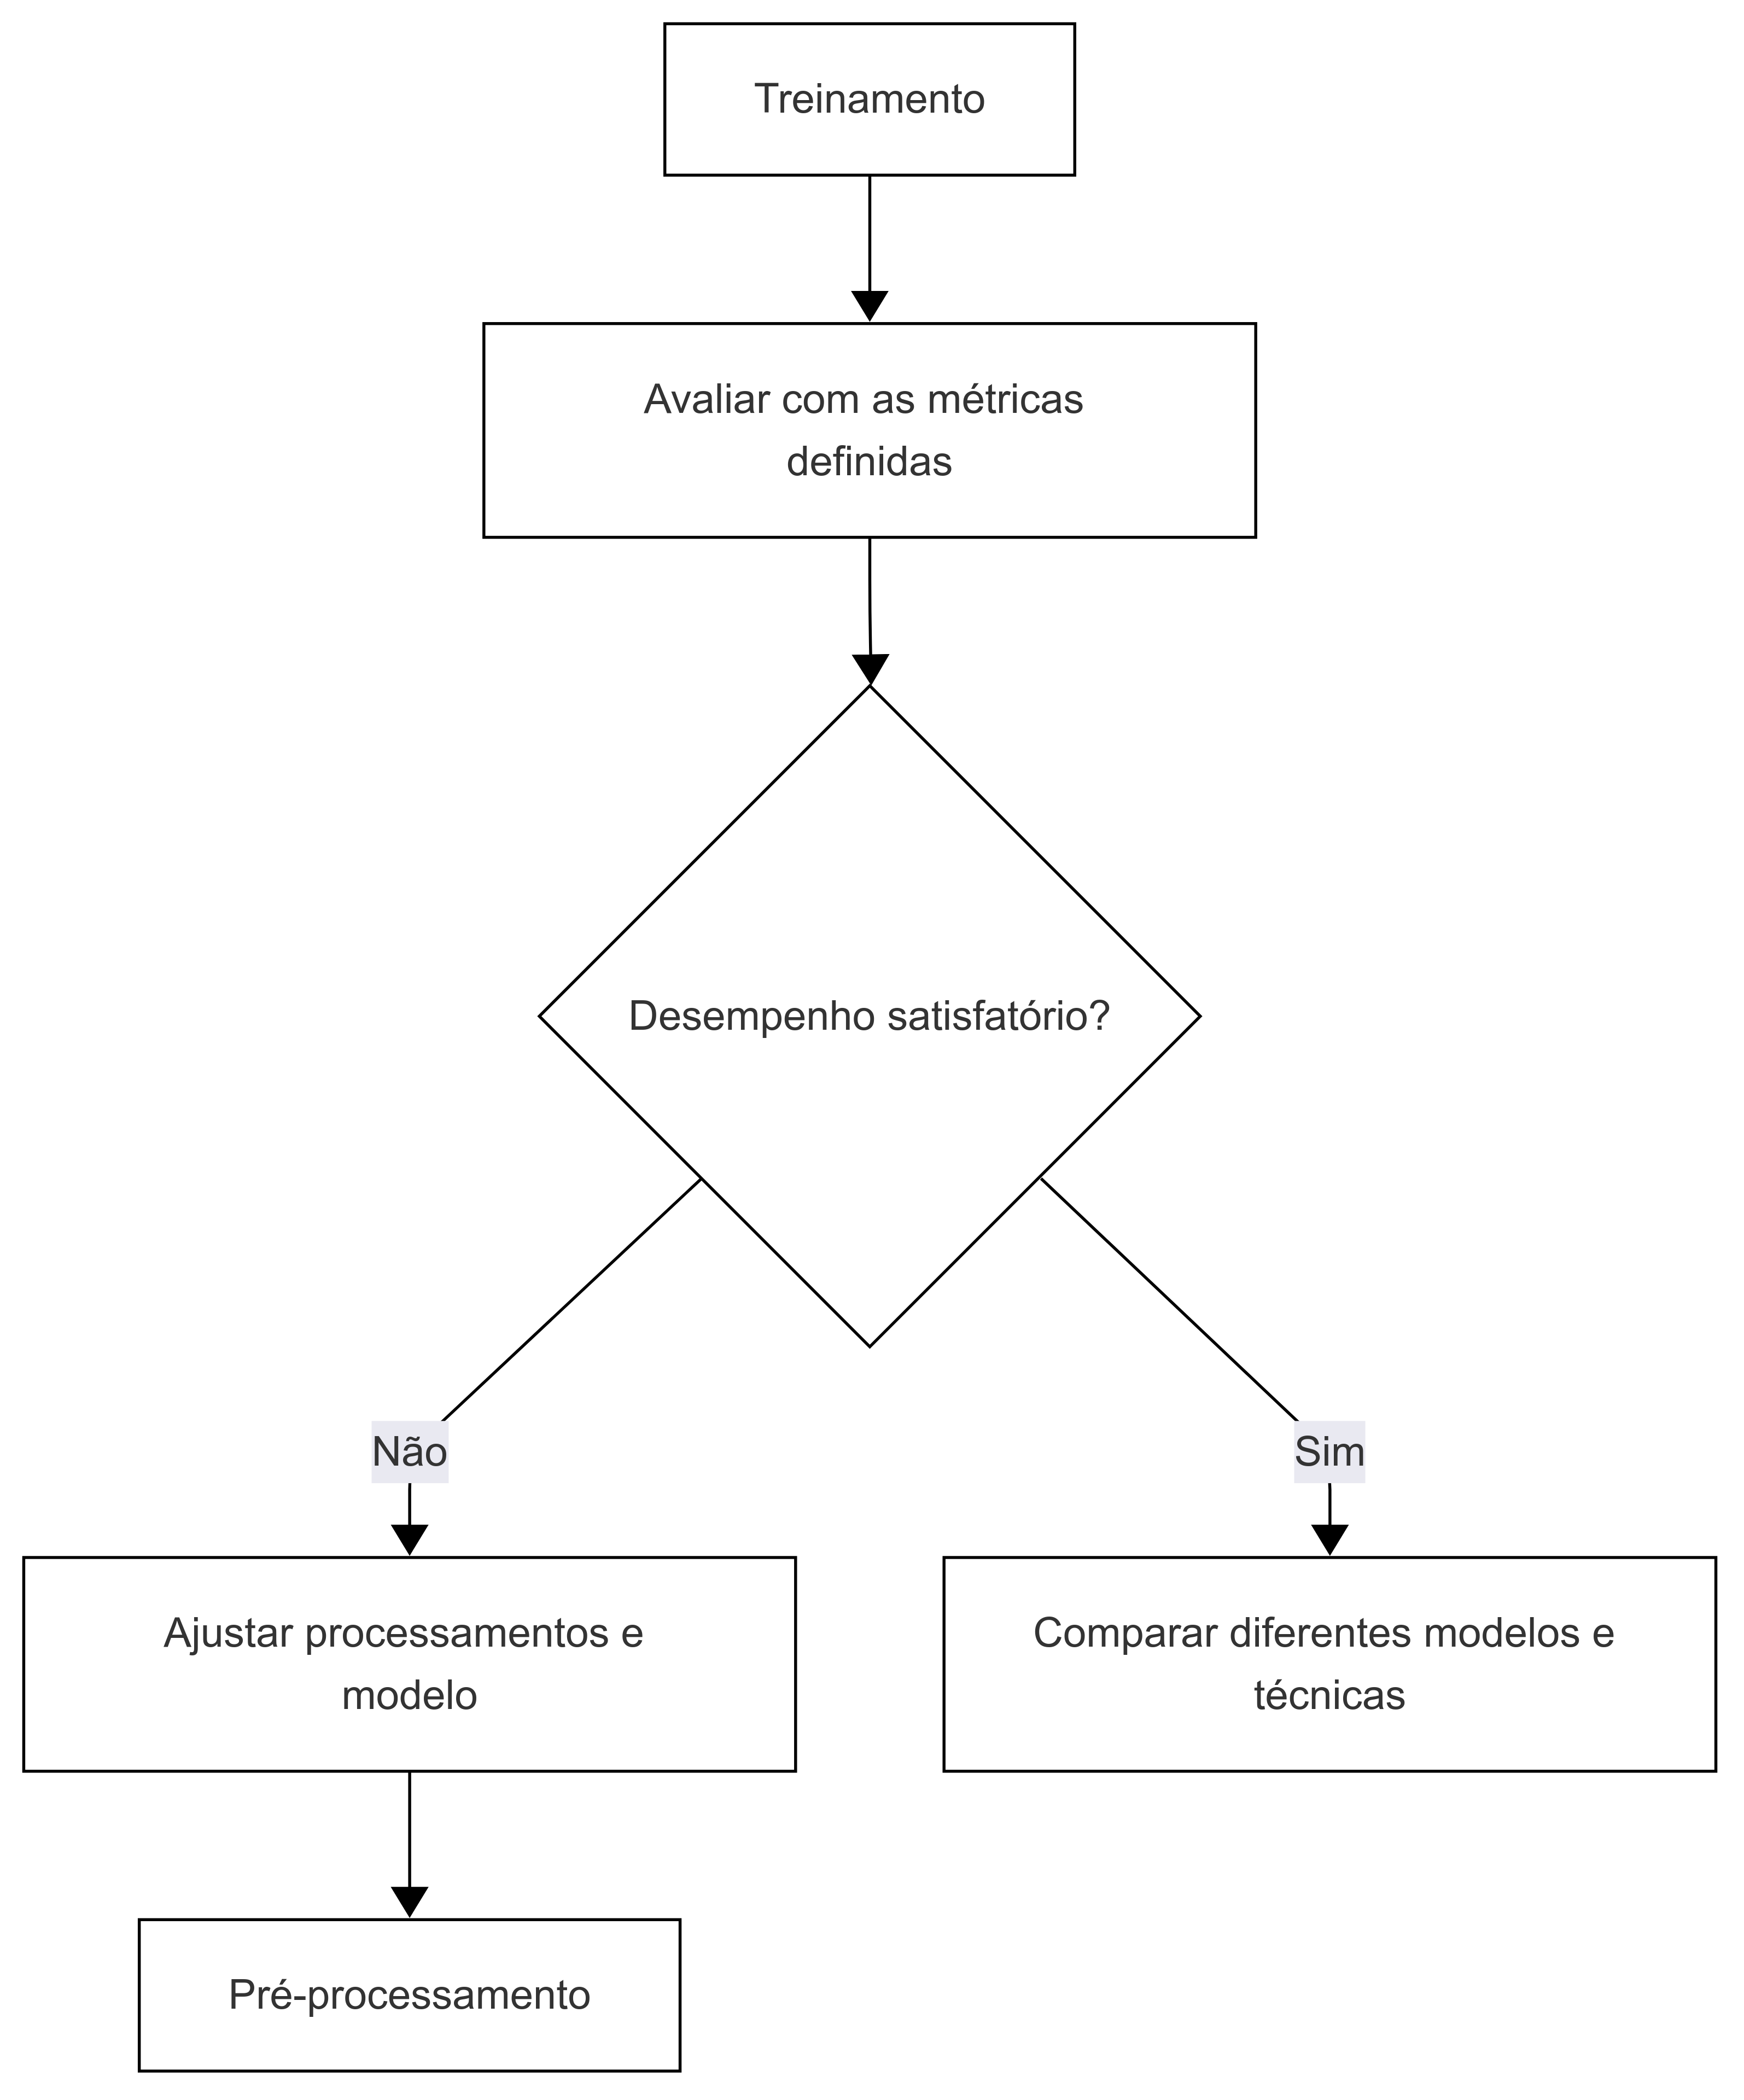
\includegraphics[width=0.85\textwidth]{img/metodologia - 6 - avaliação.png}
    \fonte{Autor.}
\end{figure}

\subsection{Avaliar com as métricas definidas}
O bloco "Avaliar com as métricas definidas" é a etapa de quantificação objetiva do desempenho do sistema utilizando as métricas estabelecidas no início da metodologia: acurácia, F1-score e tempo de processamento. A expectativa é que, nesta fase, sejam calculadas e analisadas criticamente essas métricas robustas, que oferecem uma visão multifacetada da performance do modelo treinado.

A acurácia oferece uma medida geral de correção das predições, o F1-score é especialmente valioso para datasets desbalanceados por combinar precisão e recall de forma harmônica, e o tempo de processamento é essencial para aplicações práticas onde a eficiência computacional é crítica, como na inspeção automatizada de linhas de transmissão. Para tarefas de detecção de objetos, métricas adicionais como mAP (mean Average Precision) também podem ser empregadas.

A dificuldade de execução é moderada, residindo mais na interpretação correta das métricas em diferentes contextos de problema, especialmente em face de datasets desbalanceados. O propósito dessas métricas é fornecer uma avaliação compreensiva e imparcial do quão bem o modelo está detectando e classificando as falhas, especialmente considerando que falsos negativos (falhas não detectadas) podem ter consequências graves em aplicações industriais.

\subsection{Desempenho satisfatório?}
O bloco de decisão "Desempenho satisfatório?" serve como um ponto de validação crítico na metodologia, determinando se os resultados obtidos atendem aos critérios de sucesso previamente estabelecidos. A expectativa é que esta decisão seja tomada com base nos valores das métricas definidas (acurácia, F1-score, tempo) comparados com thresholds ou benchmarks pré-estabelecidos.

Por exemplo, pode-se estabelecer que o sistema deve atingir pelo menos 95\% de acurácia, F1-score superior a 0.90 para a detecção de falhas, e tempo de processamento inferior a 100ms por imagem para ser considerado satisfatório. Esta decisão é crucial pois determina se o processo deve continuar com ajustes (caso o desempenho não seja satisfatório) ou se pode prosseguir para a fase de comparação e conclusão.

A dificuldade de execução é baixa, sendo uma decisão lógica baseada em critérios objetivos. No entanto, é fundamental que os critérios de sucesso sejam bem definidos e realistas para evitar ciclos de otimização infinitos ou conclusões prematuras.

\subsection{Ajustar processamentos e modelo}
O bloco "Ajustar processamentos e modelo" é executado quando o desempenho não é considerado satisfatório, implementando uma abordagem iterativa de refinamento. A expectativa é que esta etapa revise e modifique tanto as técnicas de processamento de imagem quanto os parâmetros do modelo de rede neural para buscar melhorias no desempenho.

Os ajustes podem envolver: revisão das técnicas de pré-processamento aplicadas, modificação dos parâmetros otimizados automaticamente, exploração de novas combinações de técnicas, ajuste fino dos hiperparâmetros do modelo de rede neural, ou até mesmo a seleção de uma arquitetura de modelo diferente. Esta etapa representa o mecanismo de feedback que permite à metodologia aprender e se adaptar com base nos resultados obtidos.

A dificuldade de execução pode ser de média a alta, dependendo da extensão dos ajustes necessários. Um erro comum é fazer modificações excessivas que comprometem o aprendizado anterior. Se os ajustes repetidos não resultarem em melhorias, as ações corretivas podem envolver uma revisão mais fundamental da abordagem, incluindo a reconsideração dos dados, da arquitetura do modelo, ou dos próprios critérios de sucesso.

\subsection{Comparar diferentes modelos e técnicas}
O bloco "Comparar diferentes modelos e técnicas" é executado quando o desempenho é considerado satisfatório, permitindo uma análise comparativa abrangente dos resultados obtidos com diferentes configurações. A expectativa é que esta etapa consolide e compare sistematicamente os resultados de todas as combinações de técnicas de processamento, parâmetros otimizados, e arquiteturas de modelos testadas ao longo da metodologia.

Esta análise comparativa é fundamental para identificar quais estratégias são mais eficazes, sob quais condições, e por quê. Inclui a comparação de métricas de desempenho, análise de trade-offs entre acurácia e velocidade, identificação de técnicas que se complementam, e documentação de insights sobre a interação entre processamentos de imagem e arquiteturas de modelos.

A dificuldade de execução é de média a alta, exigindo sólidas habilidades analíticas e conhecimento em estatística para realizar comparações significativas. A avaliação do sucesso é dada pela geração de conclusões claras sobre as abordagens mais eficazes e recomendações práticas para implementação.

\subsection{Conclusões e recomendações}
O bloco "Conclusões e recomendações" representa a fase final da metodologia, onde todo o conhecimento adquirido é consolidado em um conjunto de conclusões acionáveis e recomendações práticas. A expectativa é que esta etapa sintetize os principais achados do estudo, incluindo as técnicas de processamento de imagem mais eficazes, as combinações ótimas, o impacto das diferentes arquiteturas de modelos, e as métricas de desempenho alcançadas.

As conclusões devem ser baseadas em evidências empíricas sólidas coletadas ao longo da metodologia, enquanto as recomendações devem fornecer diretrizes práticas para implementação em cenários reais. Isso inclui a apresentação das melhores práticas identificadas, limitações observadas, e sugestões para pesquisas futuras que possam expandir o escopo do trabalho.

A dificuldade de execução é moderada, exigindo clareza na comunicação, capacidade de síntese e rigor na interpretação dos resultados. A avaliação do sucesso é medida pela completude e clareza das conclusões, e pela utilidade prática das recomendações para futuras implementações do sistema de detecção de falhas em isoladores.